\documentclass[1p]{elsarticle_modified}
%\bibliographystyle{elsarticle-num}

%\usepackage[colorlinks]{hyperref}
%\usepackage{abbrmath_seonhwa} %\Abb, \Ascr, \Acal ,\Abf, \Afrak
\usepackage{amsfonts}
\usepackage{amssymb}
\usepackage{amsmath}
\usepackage{amsthm}
\usepackage{scalefnt}
\usepackage{amsbsy}
\usepackage{kotex}
\usepackage{caption}
\usepackage{subfig}
\usepackage{color}
\usepackage{graphicx}
\usepackage{xcolor} %% white, black, red, green, blue, cyan, magenta, yellow
\usepackage{float}
\usepackage{setspace}
\usepackage{hyperref}

\usepackage{tikz}
\usetikzlibrary{arrows}

\usepackage{multirow}
\usepackage{array} % fixed length table
\usepackage{hhline}

%%%%%%%%%%%%%%%%%%%%%
\makeatletter
\renewcommand*\env@matrix[1][\arraystretch]{%
	\edef\arraystretch{#1}%
	\hskip -\arraycolsep
	\let\@ifnextchar\new@ifnextchar
	\array{*\c@MaxMatrixCols c}}
\makeatother %https://tex.stackexchange.com/questions/14071/how-can-i-increase-the-line-spacing-in-a-matrix
%%%%%%%%%%%%%%%

\usepackage[normalem]{ulem}

\newcommand{\msout}[1]{\ifmmode\text{\sout{\ensuremath{#1}}}\else\sout{#1}\fi}
%SOURCE: \msout is \stkout macro in https://tex.stackexchange.com/questions/20609/strikeout-in-math-mode

\newcommand{\cancel}[1]{
	\ifmmode
	{\color{red}\msout{#1}}
	\else
	{\color{red}\sout{#1}}
	\fi
}

\newcommand{\add}[1]{
	{\color{blue}\uwave{#1}}
}

\newcommand{\replace}[2]{
	\ifmmode
	{\color{red}\msout{#1}}{\color{blue}\uwave{#2}}
	\else
	{\color{red}\sout{#1}}{\color{blue}\uwave{#2}}
	\fi
}

\newcommand{\Sol}{\mathcal{S}} %segment
\newcommand{\D}{D} %diagram
\newcommand{\A}{\mathcal{A}} %arc


%%%%%%%%%%%%%%%%%%%%%%%%%%%%%5 test

\def\sl{\operatorname{\textup{SL}}(2,\Cbb)}
\def\psl{\operatorname{\textup{PSL}}(2,\Cbb)}
\def\quan{\mkern 1mu \triangleright \mkern 1mu}

\theoremstyle{definition}
\newtheorem{thm}{Theorem}[section]
\newtheorem{prop}[thm]{Proposition}
\newtheorem{lem}[thm]{Lemma}
\newtheorem{ques}[thm]{Question}
\newtheorem{cor}[thm]{Corollary}
\newtheorem{defn}[thm]{Definition}
\newtheorem{exam}[thm]{Example}
\newtheorem{rmk}[thm]{Remark}
\newtheorem{alg}[thm]{Algorithm}

\newcommand{\I}{\sqrt{-1}}
\begin{document}

%\begin{frontmatter}
%
%\title{Boundary parabolic representations of knots up to 8 crossings}
%
%%% Group authors per affiliation:
%\author{Yunhi Cho} 
%\address{Department of Mathematics, University of Seoul, Seoul, Korea}
%\ead{yhcho@uos.ac.kr}
%
%
%\author{Seonhwa Kim} %\fnref{s_kim}}
%\address{Center for Geometry and Physics, Institute for Basic Science, Pohang, 37673, Korea}
%\ead{ryeona17@ibs.re.kr}
%
%\author{Hyuk Kim}
%\address{Department of Mathematical Sciences, Seoul National University, Seoul 08826, Korea}
%\ead{hyukkim@snu.ac.kr}
%
%\author{Seokbeom Yoon}
%\address{Department of Mathematical Sciences, Seoul National University, Seoul, 08826,  Korea}
%\ead{sbyoon15@snu.ac.kr}
%
%\begin{abstract}
%We find all boundary parabolic representation of knots up to 8 crossings.
%
%\end{abstract}
%\begin{keyword}
%    \MSC[2010] 57M25 
%\end{keyword}
%
%\end{frontmatter}

%\linenumbers
%\tableofcontents
%
\newcommand\colored[1]{\textcolor{white}{\rule[-0.35ex]{0.8em}{1.4ex}}\kern-0.8em\color{red} #1}%
%\newcommand\colored[1]{\textcolor{white}{ #1}\kern-2.17ex	\textcolor{white}{ #1}\kern-1.81ex	\textcolor{white}{ #1}\kern-2.15ex\color{red}#1	}

{\Large $\underline{12n_{0615}~(K12n_{0615})}$}

\setlength{\tabcolsep}{10pt}
\renewcommand{\arraystretch}{1.6}
\vspace{1cm}\begin{tabular}{m{100pt}>{\centering\arraybackslash}m{274pt}}
\multirow{5}{120pt}{
	\centering
	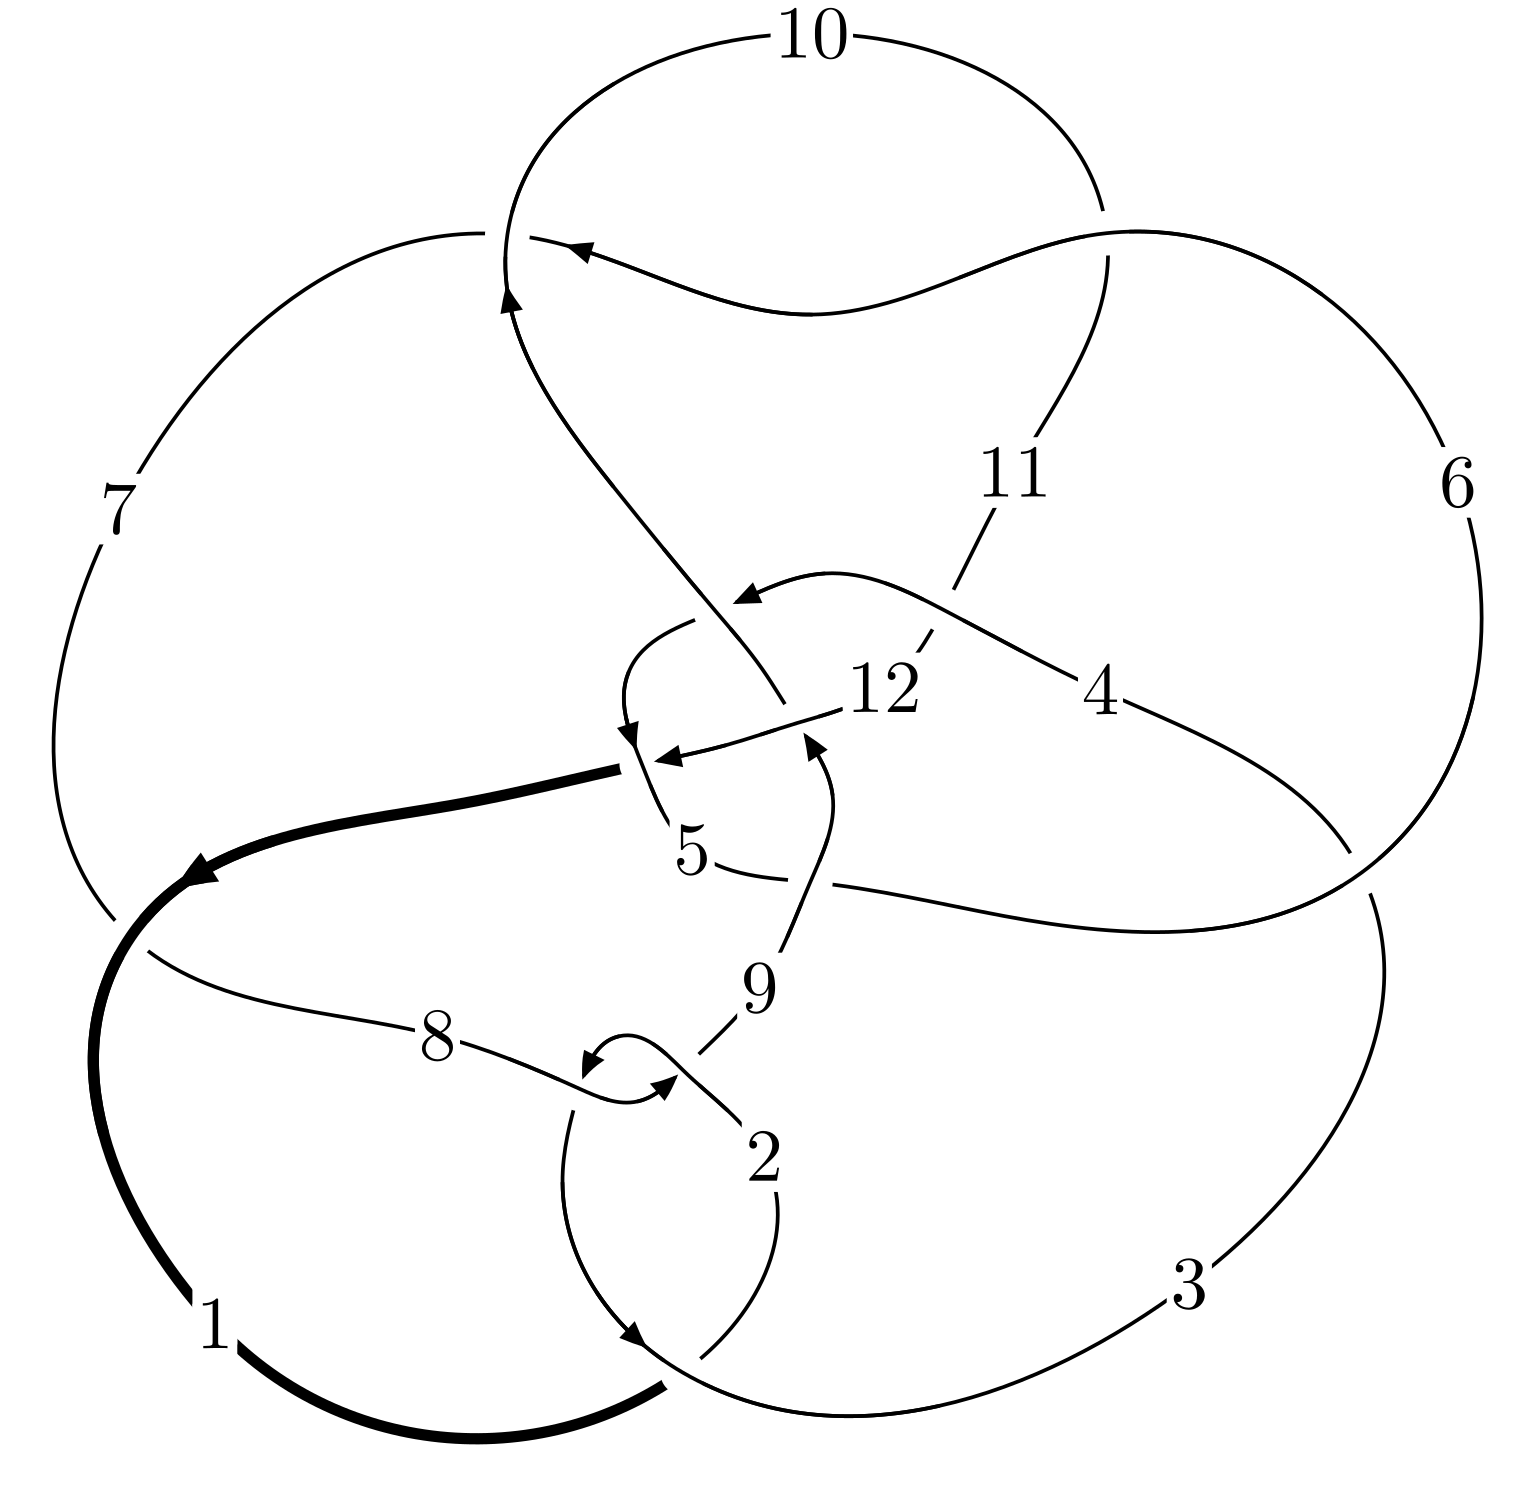
\includegraphics[width=112pt]{../../../GIT/diagram.site/Diagrams/png/2704_12n_0615.png}\\
\ \ \ A knot diagram\footnotemark}&
\allowdisplaybreaks
\textbf{Linearized knot diagam} \\
\cline{2-2}
 &
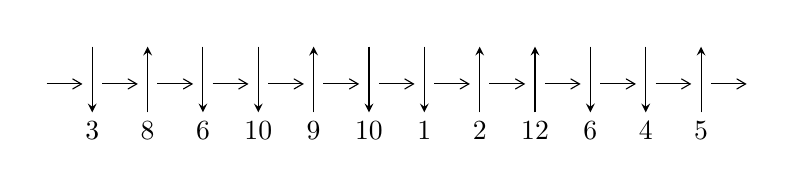
\begin{tikzpicture}[x=20pt, y=17pt]
	% nodes
	\node (C0) at (0, 0) {};
	\node (C1) at (1, 0) {};
	\node (C1U) at (1, +1) {};
	\node (C1D) at (1, -1) {3};

	\node (C2) at (2, 0) {};
	\node (C2U) at (2, +1) {};
	\node (C2D) at (2, -1) {8};

	\node (C3) at (3, 0) {};
	\node (C3U) at (3, +1) {};
	\node (C3D) at (3, -1) {6};

	\node (C4) at (4, 0) {};
	\node (C4U) at (4, +1) {};
	\node (C4D) at (4, -1) {10};

	\node (C5) at (5, 0) {};
	\node (C5U) at (5, +1) {};
	\node (C5D) at (5, -1) {9};

	\node (C6) at (6, 0) {};
	\node (C6U) at (6, +1) {};
	\node (C6D) at (6, -1) {10};

	\node (C7) at (7, 0) {};
	\node (C7U) at (7, +1) {};
	\node (C7D) at (7, -1) {1};

	\node (C8) at (8, 0) {};
	\node (C8U) at (8, +1) {};
	\node (C8D) at (8, -1) {2};

	\node (C9) at (9, 0) {};
	\node (C9U) at (9, +1) {};
	\node (C9D) at (9, -1) {12};

	\node (C10) at (10, 0) {};
	\node (C10U) at (10, +1) {};
	\node (C10D) at (10, -1) {6};

	\node (C11) at (11, 0) {};
	\node (C11U) at (11, +1) {};
	\node (C11D) at (11, -1) {4};

	\node (C12) at (12, 0) {};
	\node (C12U) at (12, +1) {};
	\node (C12D) at (12, -1) {5};
	\node (C13) at (13, 0) {};

	% arrows
	\draw[->,>={angle 60}]
	(C0) edge (C1) (C1) edge (C2) (C2) edge (C3) (C3) edge (C4) (C4) edge (C5) (C5) edge (C6) (C6) edge (C7) (C7) edge (C8) (C8) edge (C9) (C9) edge (C10) (C10) edge (C11) (C11) edge (C12) (C12) edge (C13) ;	\draw[->,>=stealth]
	(C1U) edge (C1D) (C2D) edge (C2U) (C3U) edge (C3D) (C4U) edge (C4D) (C5D) edge (C5U) (C6U) edge (C6D) (C7U) edge (C7D) (C8D) edge (C8U) (C9D) edge (C9U) (C10U) edge (C10D) (C11U) edge (C11D) (C12D) edge (C12U) ;
	\end{tikzpicture} \\
\hhline{~~} \\& 
\textbf{Solving Sequence} \\ \cline{2-2} 
 &
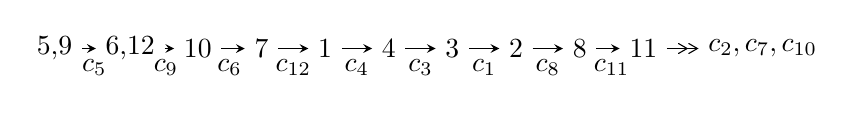
\begin{tikzpicture}[x=23pt, y=7pt]
	% node
	\node (A0) at (-1/8, 0) {5,9};
	\node (A1) at (17/16, 0) {6,12};
	\node (A2) at (17/8, 0) {10};
	\node (A3) at (25/8, 0) {7};
	\node (A4) at (33/8, 0) {1};
	\node (A5) at (41/8, 0) {4};
	\node (A6) at (49/8, 0) {3};
	\node (A7) at (57/8, 0) {2};
	\node (A8) at (65/8, 0) {8};
	\node (A9) at (73/8, 0) {11};
	\node (C1) at (1/2, -1) {$c_{5}$};
	\node (C2) at (13/8, -1) {$c_{9}$};
	\node (C3) at (21/8, -1) {$c_{6}$};
	\node (C4) at (29/8, -1) {$c_{12}$};
	\node (C5) at (37/8, -1) {$c_{4}$};
	\node (C6) at (45/8, -1) {$c_{3}$};
	\node (C7) at (53/8, -1) {$c_{1}$};
	\node (C8) at (61/8, -1) {$c_{8}$};
	\node (C9) at (69/8, -1) {$c_{11}$};
	\node (A10) at (11, 0) {$c_{2},c_{7},c_{10}$};

	% edge
	\draw[->,>=stealth]	
	(A0) edge (A1) (A1) edge (A2) (A2) edge (A3) (A3) edge (A4) (A4) edge (A5) (A5) edge (A6) (A6) edge (A7) (A7) edge (A8) (A8) edge (A9) ;
	\draw[->>,>={angle 60}]	
	(A9) edge (A10);
\end{tikzpicture} \\ 

\end{tabular} \\

\footnotetext{
The image of knot diagram is generated by the software ``\textbf{Draw programme}" developed by Andrew Bartholomew(\url{http://www.layer8.co.uk/maths/draw/index.htm\#Running-draw}), where we modified some parts for our purpose(\url{https://github.com/CATsTAILs/LinksPainter}).
}\phantom \\ \newline 
\centering \textbf{Ideals for irreducible components\footnotemark of $X_{\text{par}}$} 
 
\begin{align*}
I^u_{1}&=\langle 
b- u,\;9.22136\times10^{39} u^{35}+9.61638\times10^{39} u^{34}+\cdots+3.09061\times10^{39} a+1.18258\times10^{40},\;u^{36}+u^{35}+\cdots+u+1\rangle \\
I^u_{2}&=\langle 
b+u,\;-1.38841\times10^{20} u^{26}+1.60384\times10^{20} u^{25}+\cdots+4.99386\times10^{19} a-6.68150\times10^{19},\\
\phantom{I^u_{2}}&\phantom{= \langle  }u^{27}- u^{26}+\cdots-10 u^2-1\rangle \\
I^u_{3}&=\langle 
3.16250\times10^{115} u^{39}+8.23787\times10^{115} u^{38}+\cdots+1.00780\times10^{119} b+9.36325\times10^{117},\\
\phantom{I^u_{3}}&\phantom{= \langle  }-3.47990\times10^{101} u^{39}-7.64552\times10^{101} u^{38}+\cdots+4.09554\times10^{104} a+7.59932\times10^{103},\\
\phantom{I^u_{3}}&\phantom{= \langle  }u^{40}+3 u^{39}+\cdots+2382 u+643\rangle \\
\\
\end{align*}
\raggedright * 3 irreducible components of $\dim_{\mathbb{C}}=0$, with total 103 representations.\\
\footnotetext{All coefficients of polynomials are rational numbers. But the coefficients are sometimes approximated in decimal forms when there is not enough margin.}
\newpage
\renewcommand{\arraystretch}{1}
\centering \section*{I. $I^u_{1}= \langle b- u,\;9.22\times10^{39} u^{35}+9.62\times10^{39} u^{34}+\cdots+3.09\times10^{39} a+1.18\times10^{40},\;u^{36}+u^{35}+\cdots+u+1 \rangle$}
\flushleft \textbf{(i) Arc colorings}\\
\begin{tabular}{m{7pt} m{180pt} m{7pt} m{180pt} }
\flushright $a_{5}=$&$\begin{pmatrix}1\\0\end{pmatrix}$ \\
\flushright $a_{9}=$&$\begin{pmatrix}0\\u\end{pmatrix}$ \\
\flushright $a_{6}=$&$\begin{pmatrix}1\\- u^2\end{pmatrix}$ \\
\flushright $a_{12}=$&$\begin{pmatrix}-2.98367 u^{35}-3.11149 u^{34}+\cdots-115.302 u-3.82636\\u\end{pmatrix}$ \\
\flushright $a_{10}=$&$\begin{pmatrix}-6.16242 u^{35}-6.04552 u^{34}+\cdots-243.525 u-13.8436\\0.211237 u^{35}+0.365136 u^{34}+\cdots+4.11149 u+0.127813\end{pmatrix}$ \\
\flushright $a_{7}=$&$\begin{pmatrix}-2.38369 u^{35}-0.856037 u^{34}+\cdots-126.270 u+47.5732\\0.148878 u^{35}+0.123183 u^{34}+\cdots-0.00667650 u-0.728008\end{pmatrix}$ \\
\flushright $a_{1}=$&$\begin{pmatrix}-2.98367 u^{35}-3.11149 u^{34}+\cdots-114.302 u-3.82636\\u\end{pmatrix}$ \\
\flushright $a_{4}=$&$\begin{pmatrix}0.582610 u^{35}+0.220715 u^{34}+\cdots+37.1948 u-18.3213\\-0.0943851 u^{35}-0.0352064 u^{34}+\cdots+0.227391 u+0.366113\end{pmatrix}$ \\
\flushright $a_{3}=$&$\begin{pmatrix}0.433732 u^{35}+0.0975317 u^{34}+\cdots+37.2014 u-17.5933\\-0.254215 u^{35}-0.141930 u^{34}+\cdots+0.104208 u+0.391808\end{pmatrix}$ \\
\flushright $a_{2}=$&$\begin{pmatrix}1.66616 u^{35}+1.85078 u^{34}+\cdots+46.2547 u+8.96445\\0.0535815 u^{35}+0.110395 u^{34}+\cdots-2.21514 u+0.107894\end{pmatrix}$ \\
\flushright $a_{8}=$&$\begin{pmatrix}0.209879 u^{35}+0.404528 u^{34}+\cdots-9.69810 u+12.3718\\0.254215 u^{35}+0.141930 u^{34}+\cdots-0.104208 u-0.391808\end{pmatrix}$ \\
\flushright $a_{11}=$&$\begin{pmatrix}-6.31730 u^{35}-6.14088 u^{34}+\cdots-253.682 u-13.8545\\0.228158 u^{35}+0.419587 u^{34}+\cdots+4.01612 u+0.187326\end{pmatrix}$\\&\end{tabular}
\flushleft \textbf{(ii) Obstruction class $= -1$}\\~\\
\flushleft \textbf{(iii) Cusp Shapes $= -2.18996 u^{35}-0.638271 u^{34}+\cdots-106.713 u+50.2757$}\\~\\
\newpage\renewcommand{\arraystretch}{1}
\flushleft \textbf{(iv) u-Polynomials at the component}\newline \\
\begin{tabular}{m{50pt}|m{274pt}}
Crossings & \hspace{64pt}u-Polynomials at each crossing \\
\hline $$\begin{aligned}c_{1}\end{aligned}$$&$\begin{aligned}
&u^{36}+17 u^{35}+\cdots+896 u+256
\end{aligned}$\\
\hline $$\begin{aligned}c_{2},c_{8}\end{aligned}$$&$\begin{aligned}
&u^{36}+9 u^{35}+\cdots+128 u+16
\end{aligned}$\\
\hline $$\begin{aligned}c_{3}\end{aligned}$$&$\begin{aligned}
&u^{36}-19 u^{35}+\cdots-6400 u+1024
\end{aligned}$\\
\hline $$\begin{aligned}c_{4}\end{aligned}$$&$\begin{aligned}
&u^{36}-16 u^{34}+\cdots+115 u+42
\end{aligned}$\\
\hline $$\begin{aligned}c_{5},c_{12}\end{aligned}$$&$\begin{aligned}
&u^{36}- u^{35}+\cdots- u+1
\end{aligned}$\\
\hline $$\begin{aligned}c_{6},c_{10},c_{11}\end{aligned}$$&$\begin{aligned}
&u^{36}+u^{35}+\cdots+2 u+1
\end{aligned}$\\
\hline $$\begin{aligned}c_{7}\end{aligned}$$&$\begin{aligned}
&u^{36}-9 u^{35}+\cdots-273856 u+43216
\end{aligned}$\\
\hline $$\begin{aligned}c_{9}\end{aligned}$$&$\begin{aligned}
&u^{36}+19 u^{35}+\cdots+464 u+32
\end{aligned}$\\
\hline
\end{tabular}\\~\\
\newpage\renewcommand{\arraystretch}{1}
\flushleft \textbf{(v) Riley Polynomials at the component}\newline \\
\begin{tabular}{m{50pt}|m{274pt}}
Crossings & \hspace{64pt}Riley Polynomials at each crossing \\
\hline $$\begin{aligned}c_{1}\end{aligned}$$&$\begin{aligned}
&y^{36}+5 y^{35}+\cdots+303104 y+65536
\end{aligned}$\\
\hline $$\begin{aligned}c_{2},c_{8}\end{aligned}$$&$\begin{aligned}
&y^{36}+17 y^{35}+\cdots+896 y+256
\end{aligned}$\\
\hline $$\begin{aligned}c_{3}\end{aligned}$$&$\begin{aligned}
&y^{36}-43 y^{35}+\cdots+39911424 y+1048576
\end{aligned}$\\
\hline $$\begin{aligned}c_{4}\end{aligned}$$&$\begin{aligned}
&y^{36}-32 y^{35}+\cdots-6169 y+1764
\end{aligned}$\\
\hline $$\begin{aligned}c_{5},c_{12}\end{aligned}$$&$\begin{aligned}
&y^{36}+21 y^{35}+\cdots+103 y+1
\end{aligned}$\\
\hline $$\begin{aligned}c_{6},c_{10},c_{11}\end{aligned}$$&$\begin{aligned}
&y^{36}-59 y^{35}+\cdots-18 y+1
\end{aligned}$\\
\hline $$\begin{aligned}c_{7}\end{aligned}$$&$\begin{aligned}
&y^{36}-7 y^{35}+\cdots+320081792 y+1867622656
\end{aligned}$\\
\hline $$\begin{aligned}c_{9}\end{aligned}$$&$\begin{aligned}
&y^{36}-3 y^{35}+\cdots+15616 y+1024
\end{aligned}$\\
\hline
\end{tabular}\\~\\
\newpage\flushleft \textbf{(vi) Complex Volumes and Cusp Shapes}
$$\begin{array}{c|c|c}  
\text{Solutions to }I^u_{1}& \I (\text{vol} + \sqrt{-1}CS) & \text{Cusp shape}\\
 \hline 
\begin{aligned}
u &= -0.118220 + 0.978327 I \\
a &= \phantom{-}0.739900 + 0.147699 I \\
b &= -0.118220 + 0.978327 I\end{aligned}
 & -4.88832 - 1.24309 I & -8.27685 + 1.44633 I \\ \hline\begin{aligned}
u &= -0.118220 - 0.978327 I \\
a &= \phantom{-}0.739900 - 0.147699 I \\
b &= -0.118220 - 0.978327 I\end{aligned}
 & -4.88832 + 1.24309 I & -8.27685 - 1.44633 I \\ \hline\begin{aligned}
u &= \phantom{-}0.891670 + 0.405032 I \\
a &= -0.663932 - 0.116326 I \\
b &= \phantom{-}0.891670 + 0.405032 I\end{aligned}
 & \phantom{-}0.41304 - 2.17632 I & -2.21227 + 4.08709 I \\ \hline\begin{aligned}
u &= \phantom{-}0.891670 - 0.405032 I \\
a &= -0.663932 + 0.116326 I \\
b &= \phantom{-}0.891670 - 0.405032 I\end{aligned}
 & \phantom{-}0.41304 + 2.17632 I & -2.21227 - 4.08709 I \\ \hline\begin{aligned}
u &= -0.265738 + 0.876405 I \\
a &= \phantom{-}1.84073 + 0.78645 I \\
b &= -0.265738 + 0.876405 I\end{aligned}
 & -4.60827 - 1.82178 I & -6.48879 + 2.84582 I \\ \hline\begin{aligned}
u &= -0.265738 - 0.876405 I \\
a &= \phantom{-}1.84073 - 0.78645 I \\
b &= -0.265738 - 0.876405 I\end{aligned}
 & -4.60827 + 1.82178 I & -6.48879 - 2.84582 I \\ \hline\begin{aligned}
u &= \phantom{-}0.531923 + 0.956773 I \\
a &= -1.54750 + 0.22966 I \\
b &= \phantom{-}0.531923 + 0.956773 I\end{aligned}
 & -5.00027 + 7.84421 I & -4.73170 - 7.47375 I \\ \hline\begin{aligned}
u &= \phantom{-}0.531923 - 0.956773 I \\
a &= -1.54750 - 0.22966 I \\
b &= \phantom{-}0.531923 - 0.956773 I\end{aligned}
 & -5.00027 - 7.84421 I & -4.73170 + 7.47375 I \\ \hline\begin{aligned}
u &= \phantom{-}0.507758 + 0.970271 I \\
a &= \phantom{-}0.25842 + 1.54816 I \\
b &= \phantom{-}0.507758 + 0.970271 I\end{aligned}
 & -8.28613 + 2.69300 I & -5.21869 - 2.66219 I \\ \hline\begin{aligned}
u &= \phantom{-}0.507758 - 0.970271 I \\
a &= \phantom{-}0.25842 - 1.54816 I \\
b &= \phantom{-}0.507758 - 0.970271 I\end{aligned}
 & -8.28613 - 2.69300 I & -5.21869 + 2.66219 I\\
 \hline 
 \end{array}$$\newpage$$\begin{array}{c|c|c}  
\text{Solutions to }I^u_{1}& \I (\text{vol} + \sqrt{-1}CS) & \text{Cusp shape}\\
 \hline 
\begin{aligned}
u &= -0.862089 + 0.681772 I \\
a &= \phantom{-}0.623323 - 0.090341 I \\
b &= -0.862089 + 0.681772 I\end{aligned}
 & \phantom{-}1.34149 - 2.31581 I & -1.56931 + 2.47888 I \\ \hline\begin{aligned}
u &= -0.862089 - 0.681772 I \\
a &= \phantom{-}0.623323 + 0.090341 I \\
b &= -0.862089 - 0.681772 I\end{aligned}
 & \phantom{-}1.34149 + 2.31581 I & -1.56931 - 2.47888 I \\ \hline\begin{aligned}
u &= \phantom{-}0.149552 + 0.886635 I \\
a &= \phantom{-}0.853564 + 0.323444 I \\
b &= \phantom{-}0.149552 + 0.886635 I\end{aligned}
 & -3.37517 + 6.25769 I & -4.77547 - 7.56558 I \\ \hline\begin{aligned}
u &= \phantom{-}0.149552 - 0.886635 I \\
a &= \phantom{-}0.853564 - 0.323444 I \\
b &= \phantom{-}0.149552 - 0.886635 I\end{aligned}
 & -3.37517 - 6.25769 I & -4.77547 + 7.56558 I \\ \hline\begin{aligned}
u &= -0.037592 + 0.765146 I \\
a &= -0.949161 + 0.180834 I \\
b &= -0.037592 + 0.765146 I\end{aligned}
 & -1.05608 - 1.63487 I & -2.47499 + 3.77648 I \\ \hline\begin{aligned}
u &= -0.037592 - 0.765146 I \\
a &= -0.949161 - 0.180834 I \\
b &= -0.037592 - 0.765146 I\end{aligned}
 & -1.05608 + 1.63487 I & -2.47499 - 3.77648 I \\ \hline\begin{aligned}
u &= -0.714501 + 1.020090 I \\
a &= -0.024002 + 1.309480 I \\
b &= -0.714501 + 1.020090 I\end{aligned}
 & -11.31080 - 8.41184 I & -6.53000 + 5.72334 I \\ \hline\begin{aligned}
u &= -0.714501 - 1.020090 I \\
a &= -0.024002 - 1.309480 I \\
b &= -0.714501 - 1.020090 I\end{aligned}
 & -11.31080 + 8.41184 I & -6.53000 - 5.72334 I \\ \hline\begin{aligned}
u &= \phantom{-}0.642524 + 1.081940 I \\
a &= -0.594301 + 0.008681 I \\
b &= \phantom{-}0.642524 + 1.081940 I\end{aligned}
 & -4.41629 + 1.23501 I & -10.98929 - 1.86840 I \\ \hline\begin{aligned}
u &= \phantom{-}0.642524 - 1.081940 I \\
a &= -0.594301 - 0.008681 I \\
b &= \phantom{-}0.642524 - 1.081940 I\end{aligned}
 & -4.41629 - 1.23501 I & -10.98929 + 1.86840 I\\
 \hline 
 \end{array}$$\newpage$$\begin{array}{c|c|c}  
\text{Solutions to }I^u_{1}& \I (\text{vol} + \sqrt{-1}CS) & \text{Cusp shape}\\
 \hline 
\begin{aligned}
u &= -0.304510 + 1.244830 I \\
a &= -0.611400 + 1.161230 I \\
b &= -0.304510 + 1.244830 I\end{aligned}
 & -13.70880 + 1.48629 I & -9.47906 - 0.90947 I \\ \hline\begin{aligned}
u &= -0.304510 - 1.244830 I \\
a &= -0.611400 - 1.161230 I \\
b &= -0.304510 - 1.244830 I\end{aligned}
 & -13.70880 - 1.48629 I & -9.47906 + 0.90947 I \\ \hline\begin{aligned}
u &= -0.838328 + 1.021100 I \\
a &= \phantom{-}0.574776 - 0.036631 I \\
b &= -0.838328 + 1.021100 I\end{aligned}
 & -0.10678 - 4.05131 I & -5.35718 + 2.78187 I \\ \hline\begin{aligned}
u &= -0.838328 - 1.021100 I \\
a &= \phantom{-}0.574776 + 0.036631 I \\
b &= -0.838328 - 1.021100 I\end{aligned}
 & -0.10678 + 4.05131 I & -5.35718 - 2.78187 I \\ \hline\begin{aligned}
u &= \phantom{-}0.86929 + 1.12336 I \\
a &= -0.552780 - 0.027142 I \\
b &= \phantom{-}0.86929 + 1.12336 I\end{aligned}
 & -2.47606 + 8.95314 I & -9.63843 - 6.69810 I \\ \hline\begin{aligned}
u &= \phantom{-}0.86929 - 1.12336 I \\
a &= -0.552780 + 0.027142 I \\
b &= \phantom{-}0.86929 - 1.12336 I\end{aligned}
 & -2.47606 - 8.95314 I & -9.63843 + 6.69810 I \\ \hline\begin{aligned}
u &= \phantom{-}0.009985 + 0.390472 I \\
a &= -1.158280 - 0.683611 I \\
b &= \phantom{-}0.009985 + 0.390472 I\end{aligned}
 & -0.143687 - 1.154050 I & -1.70239 + 6.30124 I \\ \hline\begin{aligned}
u &= \phantom{-}0.009985 - 0.390472 I \\
a &= -1.158280 + 0.683611 I \\
b &= \phantom{-}0.009985 - 0.390472 I\end{aligned}
 & -0.143687 + 1.154050 I & -1.70239 - 6.30124 I \\ \hline\begin{aligned}
u &= \phantom{-}0.99600 + 1.37401 I \\
a &= -0.905942 + 0.047100 I \\
b &= \phantom{-}0.99600 + 1.37401 I\end{aligned}
 & -9.4005 + 11.0269 I & \phantom{-0.000000 } 0 \\ \hline\begin{aligned}
u &= \phantom{-}0.99600 - 1.37401 I \\
a &= -0.905942 - 0.047100 I \\
b &= \phantom{-}0.99600 - 1.37401 I\end{aligned}
 & -9.4005 - 11.0269 I & \phantom{-0.000000 } 0\\
 \hline 
 \end{array}$$\newpage$$\begin{array}{c|c|c}  
\text{Solutions to }I^u_{1}& \I (\text{vol} + \sqrt{-1}CS) & \text{Cusp shape}\\
 \hline 
\begin{aligned}
u &= -0.81790 + 1.51742 I \\
a &= \phantom{-}0.883941 + 0.187003 I \\
b &= -0.81790 + 1.51742 I\end{aligned}
 & -14.4218 - 6.9271 I & \phantom{-0.000000 } 0 \\ \hline\begin{aligned}
u &= -0.81790 - 1.51742 I \\
a &= \phantom{-}0.883941 - 0.187003 I \\
b &= -0.81790 - 1.51742 I\end{aligned}
 & -14.4218 + 6.9271 I & \phantom{-0.000000 } 0 \\ \hline\begin{aligned}
u &= -1.12027 + 1.43623 I \\
a &= \phantom{-}0.832072 + 0.016628 I \\
b &= -1.12027 + 1.43623 I\end{aligned}
 & -12.4101 - 16.4883 I & \phantom{-0.000000 } 0 \\ \hline\begin{aligned}
u &= -1.12027 - 1.43623 I \\
a &= \phantom{-}0.832072 - 0.016628 I \\
b &= -1.12027 - 1.43623 I\end{aligned}
 & -12.4101 + 16.4883 I & \phantom{-0.000000 } 0 \\ \hline\begin{aligned}
u &= -0.019556 + 0.157716 I \\
a &= -3.59942 - 13.15270 I \\
b &= -0.019556 + 0.157716 I\end{aligned}
 & \phantom{-}5.85065 - 3.09111 I & \phantom{-}34.3315 - 14.8344 I \\ \hline\begin{aligned}
u &= -0.019556 - 0.157716 I \\
a &= -3.59942 + 13.15270 I \\
b &= -0.019556 - 0.157716 I\end{aligned}
 & \phantom{-}5.85065 + 3.09111 I & \phantom{-}34.3315 + 14.8344 I\\
 \hline 
 \end{array}$$\newpage\newpage\renewcommand{\arraystretch}{1}
\centering \section*{II. $I^u_{2}= \langle b+u,\;-1.39\times10^{20} u^{26}+1.60\times10^{20} u^{25}+\cdots+4.99\times10^{19} a-6.68\times10^{19},\;u^{27}- u^{26}+\cdots-10 u^2-1 \rangle$}
\flushleft \textbf{(i) Arc colorings}\\
\begin{tabular}{m{7pt} m{180pt} m{7pt} m{180pt} }
\flushright $a_{5}=$&$\begin{pmatrix}1\\0\end{pmatrix}$ \\
\flushright $a_{9}=$&$\begin{pmatrix}0\\u\end{pmatrix}$ \\
\flushright $a_{6}=$&$\begin{pmatrix}1\\- u^2\end{pmatrix}$ \\
\flushright $a_{12}=$&$\begin{pmatrix}2.78024 u^{26}-3.21163 u^{25}+\cdots-21.1050 u+1.33794\\- u\end{pmatrix}$ \\
\flushright $a_{10}=$&$\begin{pmatrix}5.30922 u^{26}-6.52376 u^{25}+\cdots-42.9670 u+0.261911\\0.295368 u^{26}-0.301221 u^{25}+\cdots-1.78024 u+0.431384\end{pmatrix}$ \\
\flushright $a_{7}=$&$\begin{pmatrix}-1.33794 u^{26}-1.44230 u^{25}+\cdots-15.2069 u+22.1050\\0.341753 u^{26}-0.265611 u^{25}+\cdots-0.783163 u+0.688731\end{pmatrix}$ \\
\flushright $a_{1}=$&$\begin{pmatrix}2.78024 u^{26}-3.21163 u^{25}+\cdots-22.1050 u+1.33794\\- u\end{pmatrix}$ \\
\flushright $a_{4}=$&$\begin{pmatrix}0.431384 u^{26}-1.13602 u^{25}+\cdots-7.33794 u+8.21976\\-0.335900 u^{26}+0.248427 u^{25}+\cdots+0.351779 u+0.0159013\end{pmatrix}$ \\
\flushright $a_{3}=$&$\begin{pmatrix}0.0896309 u^{26}-0.870405 u^{25}+\cdots-6.55478 u+7.53103\\-0.418450 u^{26}+0.307498 u^{25}+\cdots+0.693532 u+0.0920432\end{pmatrix}$ \\
\flushright $a_{2}=$&$\begin{pmatrix}-1.05574 u^{26}+1.20442 u^{25}+\cdots+7.08036 u+1.76225\\-0.0188017 u^{26}-0.271955 u^{25}+\cdots-0.0680159 u+0.737192\end{pmatrix}$ \\
\flushright $a_{8}=$&$\begin{pmatrix}-1.14370 u^{26}+0.583208 u^{25}+\cdots+0.782926 u+4.82381\\0.418450 u^{26}-0.307498 u^{25}+\cdots-0.693532 u-0.0920432\end{pmatrix}$ \\
\flushright $a_{11}=$&$\begin{pmatrix}5.62049 u^{26}-7.17679 u^{25}+\cdots-46.4959 u+1.04507\\0.371510 u^{26}-0.459914 u^{25}+\cdots-2.09151 u+0.773138\end{pmatrix}$\\&\end{tabular}
\flushleft \textbf{(ii) Obstruction class $= 1$}\\~\\
\flushleft \textbf{(iii) Cusp Shapes $= \frac{62283098744443613578}{49938603651971298581} u^{26}+\frac{232496535338997910625}{49938603651971298581} u^{25}+\cdots+\frac{2030283186351200219352}{49938603651971298581} u-\frac{2398399780063016104203}{49938603651971298581}$}\\~\\
\newpage\renewcommand{\arraystretch}{1}
\flushleft \textbf{(iv) u-Polynomials at the component}\newline \\
\begin{tabular}{m{50pt}|m{274pt}}
Crossings & \hspace{64pt}u-Polynomials at each crossing \\
\hline $$\begin{aligned}c_{1}\end{aligned}$$&$\begin{aligned}
&u^{27}-14 u^{26}+\cdots-8 u+1
\end{aligned}$\\
\hline $$\begin{aligned}c_{2}\end{aligned}$$&$\begin{aligned}
&u^{27}+7 u^{25}+\cdots+4 u^2+1
\end{aligned}$\\
\hline $$\begin{aligned}c_{3}\end{aligned}$$&$\begin{aligned}
&u^{27}-20 u^{26}+\cdots+413 u-181
\end{aligned}$\\
\hline $$\begin{aligned}c_{4}\end{aligned}$$&$\begin{aligned}
&u^{27}-6 u^{25}+\cdots+14 u-5
\end{aligned}$\\
\hline $$\begin{aligned}c_{5},c_{12}\end{aligned}$$&$\begin{aligned}
&u^{27}- u^{26}+\cdots-10 u^2-1
\end{aligned}$\\
\hline $$\begin{aligned}c_{6},c_{11}\end{aligned}$$&$\begin{aligned}
&u^{27}+u^{26}+\cdots- u-1
\end{aligned}$\\
\hline $$\begin{aligned}c_{7}\end{aligned}$$&$\begin{aligned}
&u^{27}- u^{25}+\cdots+12 u-5
\end{aligned}$\\
\hline $$\begin{aligned}c_{8}\end{aligned}$$&$\begin{aligned}
&u^{27}+7 u^{25}+\cdots-4 u^2-1
\end{aligned}$\\
\hline $$\begin{aligned}c_{9}\end{aligned}$$&$\begin{aligned}
&u^{27}+12 u^{26}+\cdots+5 u^2-1
\end{aligned}$\\
\hline $$\begin{aligned}c_{10}\end{aligned}$$&$\begin{aligned}
&u^{27}- u^{26}+\cdots- u+1
\end{aligned}$\\
\hline
\end{tabular}\\~\\
\newpage\renewcommand{\arraystretch}{1}
\flushleft \textbf{(v) Riley Polynomials at the component}\newline \\
\begin{tabular}{m{50pt}|m{274pt}}
Crossings & \hspace{64pt}Riley Polynomials at each crossing \\
\hline $$\begin{aligned}c_{1}\end{aligned}$$&$\begin{aligned}
&y^{27}+6 y^{26}+\cdots-8 y-1
\end{aligned}$\\
\hline $$\begin{aligned}c_{2},c_{8}\end{aligned}$$&$\begin{aligned}
&y^{27}+14 y^{26}+\cdots-8 y-1
\end{aligned}$\\
\hline $$\begin{aligned}c_{3}\end{aligned}$$&$\begin{aligned}
&y^{27}-36 y^{26}+\cdots+599539 y-32761
\end{aligned}$\\
\hline $$\begin{aligned}c_{4}\end{aligned}$$&$\begin{aligned}
&y^{27}-12 y^{26}+\cdots-34 y-25
\end{aligned}$\\
\hline $$\begin{aligned}c_{5},c_{12}\end{aligned}$$&$\begin{aligned}
&y^{27}-7 y^{26}+\cdots-20 y-1
\end{aligned}$\\
\hline $$\begin{aligned}c_{6},c_{10},c_{11}\end{aligned}$$&$\begin{aligned}
&y^{27}-15 y^{26}+\cdots-19 y-1
\end{aligned}$\\
\hline $$\begin{aligned}c_{7}\end{aligned}$$&$\begin{aligned}
&y^{27}-2 y^{26}+\cdots-236 y-25
\end{aligned}$\\
\hline $$\begin{aligned}c_{9}\end{aligned}$$&$\begin{aligned}
&y^{27}-4 y^{26}+\cdots+10 y-1
\end{aligned}$\\
\hline
\end{tabular}\\~\\
\newpage\flushleft \textbf{(vi) Complex Volumes and Cusp Shapes}
$$\begin{array}{c|c|c}  
\text{Solutions to }I^u_{2}& \I (\text{vol} + \sqrt{-1}CS) & \text{Cusp shape}\\
 \hline 
\begin{aligned}
u &= -0.336357 + 0.966243 I \\
a &= -0.686667 + 0.398689 I \\
b &= \phantom{-}0.336357 - 0.966243 I\end{aligned}
 & -6.68205 - 0.58234 I & -13.57427 + 1.26764 I \\ \hline\begin{aligned}
u &= -0.336357 - 0.966243 I \\
a &= -0.686667 - 0.398689 I \\
b &= \phantom{-}0.336357 + 0.966243 I\end{aligned}
 & -6.68205 + 0.58234 I & -13.57427 - 1.26764 I \\ \hline\begin{aligned}
u &= -1.005400 + 0.275951 I \\
a &= -1.037330 + 0.705161 I \\
b &= \phantom{-}1.005400 - 0.275951 I\end{aligned}
 & \phantom{-}1.83930 - 2.45917 I & \phantom{-}1.80526 + 7.62829 I \\ \hline\begin{aligned}
u &= -1.005400 - 0.275951 I \\
a &= -1.037330 - 0.705161 I \\
b &= \phantom{-}1.005400 + 0.275951 I\end{aligned}
 & \phantom{-}1.83930 + 2.45917 I & \phantom{-}1.80526 - 7.62829 I \\ \hline\begin{aligned}
u &= \phantom{-}0.606745 + 0.882798 I \\
a &= \phantom{-}0.331286 + 0.517855 I \\
b &= -0.606745 - 0.882798 I\end{aligned}
 & -5.64281 - 2.15614 I & -9.19261 - 1.44075 I \\ \hline\begin{aligned}
u &= \phantom{-}0.606745 - 0.882798 I \\
a &= \phantom{-}0.331286 - 0.517855 I \\
b &= -0.606745 + 0.882798 I\end{aligned}
 & -5.64281 + 2.15614 I & -9.19261 + 1.44075 I \\ \hline\begin{aligned}
u &= \phantom{-}1.07541\phantom{ +0.000000I} \\
a &= -0.461440\phantom{ +0.000000I} \\
b &= -1.07541\phantom{ +0.000000I}\end{aligned}
 & -7.12921\phantom{ +0.000000I} & -4.03220\phantom{ +0.000000I} \\ \hline\begin{aligned}
u &= \phantom{-}0.537424 + 1.012470 I \\
a &= \phantom{-}0.721465 - 0.486432 I \\
b &= -0.537424 - 1.012470 I\end{aligned}
 & -3.11876 + 0.97105 I & -4.34103 - 1.79332 I \\ \hline\begin{aligned}
u &= \phantom{-}0.537424 - 1.012470 I \\
a &= \phantom{-}0.721465 + 0.486432 I \\
b &= -0.537424 + 1.012470 I\end{aligned}
 & -3.11876 - 0.97105 I & -4.34103 + 1.79332 I \\ \hline\begin{aligned}
u &= -0.816309 + 0.907921 I \\
a &= -0.862083 - 0.153746 I \\
b &= \phantom{-}0.816309 - 0.907921 I\end{aligned}
 & \phantom{-}1.00458 - 4.33611 I & \phantom{-}2.54294 + 5.25647 I\\
 \hline 
 \end{array}$$\newpage$$\begin{array}{c|c|c}  
\text{Solutions to }I^u_{2}& \I (\text{vol} + \sqrt{-1}CS) & \text{Cusp shape}\\
 \hline 
\begin{aligned}
u &= -0.816309 - 0.907921 I \\
a &= -0.862083 + 0.153746 I \\
b &= \phantom{-}0.816309 + 0.907921 I\end{aligned}
 & \phantom{-}1.00458 + 4.33611 I & \phantom{-}2.54294 - 5.25647 I \\ \hline\begin{aligned}
u &= \phantom{-}1.216070 + 0.287083 I \\
a &= \phantom{-}0.772680 + 0.609470 I \\
b &= -1.216070 - 0.287083 I\end{aligned}
 & \phantom{-}0.51517 + 5.99705 I & -4.48976 - 8.64665 I \\ \hline\begin{aligned}
u &= \phantom{-}1.216070 - 0.287083 I \\
a &= \phantom{-}0.772680 - 0.609470 I \\
b &= -1.216070 + 0.287083 I\end{aligned}
 & \phantom{-}0.51517 - 5.99705 I & -4.48976 + 8.64665 I \\ \hline\begin{aligned}
u &= -1.127710 + 0.614247 I \\
a &= -0.861605 + 0.280734 I \\
b &= \phantom{-}1.127710 - 0.614247 I\end{aligned}
 & \phantom{-}2.32898 - 3.69540 I & \phantom{-}1.96062 + 2.95334 I \\ \hline\begin{aligned}
u &= -1.127710 - 0.614247 I \\
a &= -0.861605 - 0.280734 I \\
b &= \phantom{-}1.127710 + 0.614247 I\end{aligned}
 & \phantom{-}2.32898 + 3.69540 I & \phantom{-}1.96062 - 2.95334 I \\ \hline\begin{aligned}
u &= -0.079298 + 0.699557 I \\
a &= -1.57234 + 0.54120 I \\
b &= \phantom{-}0.079298 - 0.699557 I\end{aligned}
 & -5.11145 + 5.51494 I & -8.41780 - 5.72397 I \\ \hline\begin{aligned}
u &= -0.079298 - 0.699557 I \\
a &= -1.57234 - 0.54120 I \\
b &= \phantom{-}0.079298 + 0.699557 I\end{aligned}
 & -5.11145 - 5.51494 I & -8.41780 + 5.72397 I \\ \hline\begin{aligned}
u &= -1.326360 + 0.260463 I \\
a &= \phantom{-}0.244005 + 0.122908 I \\
b &= \phantom{-}1.326360 - 0.260463 I\end{aligned}
 & -10.69710 + 4.45935 I & -7.92473 - 3.01900 I \\ \hline\begin{aligned}
u &= -1.326360 - 0.260463 I \\
a &= \phantom{-}0.244005 - 0.122908 I \\
b &= \phantom{-}1.326360 + 0.260463 I\end{aligned}
 & -10.69710 - 4.45935 I & -7.92473 + 3.01900 I \\ \hline\begin{aligned}
u &= \phantom{-}0.859553 + 1.069800 I \\
a &= \phantom{-}0.705680 - 0.146031 I \\
b &= -0.859553 - 1.069800 I\end{aligned}
 & -1.59462 + 9.09497 I & -0.27825 - 8.37177 I\\
 \hline 
 \end{array}$$\newpage$$\begin{array}{c|c|c}  
\text{Solutions to }I^u_{2}& \I (\text{vol} + \sqrt{-1}CS) & \text{Cusp shape}\\
 \hline 
\begin{aligned}
u &= \phantom{-}0.859553 - 1.069800 I \\
a &= \phantom{-}0.705680 + 0.146031 I \\
b &= -0.859553 + 1.069800 I\end{aligned}
 & -1.59462 - 9.09497 I & -0.27825 + 8.37177 I \\ \hline\begin{aligned}
u &= \phantom{-}1.286270 + 0.526184 I \\
a &= \phantom{-}0.741479 + 0.383886 I \\
b &= -1.286270 - 0.526184 I\end{aligned}
 & \phantom{-}0.771357 - 0.260360 I & -4.29150 + 1.30501 I \\ \hline\begin{aligned}
u &= \phantom{-}1.286270 - 0.526184 I \\
a &= \phantom{-}0.741479 - 0.383886 I \\
b &= -1.286270 + 0.526184 I\end{aligned}
 & \phantom{-}0.771357 + 0.260360 I & -4.29150 - 1.30501 I \\ \hline\begin{aligned}
u &= \phantom{-}0.221536 + 0.540952 I \\
a &= \phantom{-}1.34818 + 1.58969 I \\
b &= -0.221536 - 0.540952 I\end{aligned}
 & -3.77045 - 0.62259 I & -2.79230 - 0.12381 I \\ \hline\begin{aligned}
u &= \phantom{-}0.221536 - 0.540952 I \\
a &= \phantom{-}1.34818 - 1.58969 I \\
b &= -0.221536 + 0.540952 I\end{aligned}
 & -3.77045 + 0.62259 I & -2.79230 + 0.12381 I \\ \hline\begin{aligned}
u &= -0.073870 + 0.346449 I \\
a &= -2.11404 - 5.83905 I \\
b &= \phantom{-}0.073870 - 0.346449 I\end{aligned}
 & \phantom{-}5.75856 - 3.13863 I & -34.4905 + 20.3622 I \\ \hline\begin{aligned}
u &= -0.073870 - 0.346449 I \\
a &= -2.11404 + 5.83905 I \\
b &= \phantom{-}0.073870 + 0.346449 I\end{aligned}
 & \phantom{-}5.75856 + 3.13863 I & -34.4905 - 20.3622 I\\
 \hline 
 \end{array}$$\newpage\newpage\renewcommand{\arraystretch}{1}
\centering \section*{III. $I^u_{3}= \langle 3.16\times10^{115} u^{39}+8.24\times10^{115} u^{38}+\cdots+1.01\times10^{119} b+9.36\times10^{117},\;-3.48\times10^{101} u^{39}-7.65\times10^{101} u^{38}+\cdots+4.10\times10^{104} a+7.60\times10^{103},\;u^{40}+3 u^{39}+\cdots+2382 u+643 \rangle$}
\flushleft \textbf{(i) Arc colorings}\\
\begin{tabular}{m{7pt} m{180pt} m{7pt} m{180pt} }
\flushright $a_{5}=$&$\begin{pmatrix}1\\0\end{pmatrix}$ \\
\flushright $a_{9}=$&$\begin{pmatrix}0\\u\end{pmatrix}$ \\
\flushright $a_{6}=$&$\begin{pmatrix}1\\- u^2\end{pmatrix}$ \\
\flushright $a_{12}=$&$\begin{pmatrix}0.000849679 u^{39}+0.00186679 u^{38}+\cdots+6.51068 u-0.185551\\-0.000313802 u^{39}-0.000817408 u^{38}+\cdots-4.43952 u-0.0929075\end{pmatrix}$ \\
\flushright $a_{10}=$&$\begin{pmatrix}0.000285297 u^{39}+0.000692402 u^{38}+\cdots-1.15794 u+2.02510\\-0.000188165 u^{39}-0.000867240 u^{38}+\cdots-0.373964 u-1.49124\end{pmatrix}$ \\
\flushright $a_{7}=$&$\begin{pmatrix}0.0000666790 u^{39}+0.000133987 u^{38}+\cdots+1.52511 u-1.95131\\0.000373461 u^{39}+0.00130423 u^{38}+\cdots-0.762077 u+1.71070\end{pmatrix}$ \\
\flushright $a_{1}=$&$\begin{pmatrix}0.000535877 u^{39}+0.00104938 u^{38}+\cdots+2.07116 u-0.278459\\-0.000313802 u^{39}-0.000817408 u^{38}+\cdots-4.43952 u-0.0929075\end{pmatrix}$ \\
\flushright $a_{4}=$&$\begin{pmatrix}0.000306782 u^{39}+0.00117024 u^{38}+\cdots-2.28718 u+3.66201\\-0.000336059 u^{39}-0.00126654 u^{38}+\cdots+1.55459 u-1.55002\end{pmatrix}$ \\
\flushright $a_{3}=$&$\begin{pmatrix}-0.0000666790 u^{39}-0.000133987 u^{38}+\cdots-1.52511 u+1.95131\\-0.000531243 u^{39}-0.00193316 u^{38}+\cdots+0.876534 u-1.66823\end{pmatrix}$ \\
\flushright $a_{2}=$&$\begin{pmatrix}0.000887834 u^{39}+0.00224028 u^{38}+\cdots+8.02399 u-0.145440\\-0.000846462 u^{39}-0.00202870 u^{38}+\cdots-6.96651 u+0.487391\end{pmatrix}$ \\
\flushright $a_{8}=$&$\begin{pmatrix}-0.000654257 u^{39}-0.00227174 u^{38}+\cdots-0.869104 u-2.95403\\0.000283061 u^{39}+0.000673324 u^{38}+\cdots+1.04746 u+2.51922\end{pmatrix}$ \\
\flushright $a_{11}=$&$\begin{pmatrix}0.000643096 u^{39}+0.00183202 u^{38}+\cdots-0.989966 u+3.41122\\-0.000105609 u^{39}-0.000634796 u^{38}+\cdots+0.0138282 u-1.44866\end{pmatrix}$\\&\end{tabular}
\flushleft \textbf{(ii) Obstruction class $= -1$}\\~\\
\flushleft \textbf{(iii) Cusp Shapes $= -0.00357512 u^{39}-0.0100039 u^{38}+\cdots-28.2430 u-9.94034$}\\~\\
\newpage\renewcommand{\arraystretch}{1}
\flushleft \textbf{(iv) u-Polynomials at the component}\newline \\
\begin{tabular}{m{50pt}|m{274pt}}
Crossings & \hspace{64pt}u-Polynomials at each crossing \\
\hline $$\begin{aligned}c_{1}\end{aligned}$$&$\begin{aligned}
&(u^5+3 u^4+4 u^3+u^2- u-1)^8
\end{aligned}$\\
\hline $$\begin{aligned}c_{2},c_{8}\end{aligned}$$&$\begin{aligned}
&(u^5- u^4+2 u^3- u^2+u-1)^8
\end{aligned}$\\
\hline $$\begin{aligned}c_{3}\end{aligned}$$&$\begin{aligned}
&(u^4+3 u^3+u^2-2 u+1)^{10}
\end{aligned}$\\
\hline $$\begin{aligned}c_{4}\end{aligned}$$&$\begin{aligned}
&u^{40}- u^{39}+\cdots-525220 u+436829
\end{aligned}$\\
\hline $$\begin{aligned}c_{5},c_{12}\end{aligned}$$&$\begin{aligned}
&u^{40}-3 u^{39}+\cdots-2382 u+643
\end{aligned}$\\
\hline $$\begin{aligned}c_{6},c_{10},c_{11}\end{aligned}$$&$\begin{aligned}
&u^{40}- u^{39}+\cdots+60966 u+88157
\end{aligned}$\\
\hline $$\begin{aligned}c_{7}\end{aligned}$$&$\begin{aligned}
&(u^5+u^4-2 u^3- u^2+u-1)^8
\end{aligned}$\\
\hline $$\begin{aligned}c_{9}\end{aligned}$$&$\begin{aligned}
&(u^4- u^3+u^2+1)^{10}
\end{aligned}$\\
\hline
\end{tabular}\\~\\
\newpage\renewcommand{\arraystretch}{1}
\flushleft \textbf{(v) Riley Polynomials at the component}\newline \\
\begin{tabular}{m{50pt}|m{274pt}}
Crossings & \hspace{64pt}Riley Polynomials at each crossing \\
\hline $$\begin{aligned}c_{1}\end{aligned}$$&$\begin{aligned}
&(y^5- y^4+8 y^3-3 y^2+3 y-1)^8
\end{aligned}$\\
\hline $$\begin{aligned}c_{2},c_{8}\end{aligned}$$&$\begin{aligned}
&(y^5+3 y^4+4 y^3+y^2- y-1)^8
\end{aligned}$\\
\hline $$\begin{aligned}c_{3}\end{aligned}$$&$\begin{aligned}
&(y^4-7 y^3+15 y^2-2 y+1)^{10}
\end{aligned}$\\
\hline $$\begin{aligned}c_{4}\end{aligned}$$&$\begin{aligned}
&y^{40}-25 y^{39}+\cdots-458444454794 y+190819575241
\end{aligned}$\\
\hline $$\begin{aligned}c_{5},c_{12}\end{aligned}$$&$\begin{aligned}
&y^{40}-5 y^{39}+\cdots+1465948 y+413449
\end{aligned}$\\
\hline $$\begin{aligned}c_{6},c_{10},c_{11}\end{aligned}$$&$\begin{aligned}
&y^{40}-45 y^{39}+\cdots-9888901040 y+7771656649
\end{aligned}$\\
\hline $$\begin{aligned}c_{7}\end{aligned}$$&$\begin{aligned}
&(y^5-5 y^4+8 y^3-3 y^2- y-1)^8
\end{aligned}$\\
\hline $$\begin{aligned}c_{9}\end{aligned}$$&$\begin{aligned}
&(y^4+y^3+3 y^2+2 y+1)^{10}
\end{aligned}$\\
\hline
\end{tabular}\\~\\
\newpage\flushleft \textbf{(vi) Complex Volumes and Cusp Shapes}
$$\begin{array}{c|c|c}  
\text{Solutions to }I^u_{3}& \I (\text{vol} + \sqrt{-1}CS) & \text{Cusp shape}\\
 \hline 
\begin{aligned}
u &= \phantom{-}0.915348 + 0.214144 I \\
a &= -0.189845 + 0.831374 I \\
b &= -0.106490 - 1.134420 I\end{aligned}
 & -5.47491 + 0.11547 I & -6.34185 + 0.47809 I \\ \hline\begin{aligned}
u &= \phantom{-}0.915348 - 0.214144 I \\
a &= -0.189845 - 0.831374 I \\
b &= -0.106490 + 1.134420 I\end{aligned}
 & -5.47491 - 0.11547 I & -6.34185 - 0.47809 I \\ \hline\begin{aligned}
u &= -0.683982 + 0.623025 I \\
a &= \phantom{-}0.805406 - 0.319531 I \\
b &= -1.92283 - 1.60754 I\end{aligned}
 & -11.01840 - 5.81594 I & -10.57105 + 8.40733 I \\ \hline\begin{aligned}
u &= -0.683982 - 0.623025 I \\
a &= \phantom{-}0.805406 + 0.319531 I \\
b &= -1.92283 + 1.60754 I\end{aligned}
 & -11.01840 + 5.81594 I & -10.57105 - 8.40733 I \\ \hline\begin{aligned}
u &= \phantom{-}1.078690 + 0.106927 I \\
a &= \phantom{-}0.864918 + 0.759081 I \\
b &= -1.023340 - 0.427389 I\end{aligned}
 & \phantom{-}1.52684 + 1.63338 I & -2.68838 + 1.86585 I \\ \hline\begin{aligned}
u &= \phantom{-}1.078690 - 0.106927 I \\
a &= \phantom{-}0.864918 - 0.759081 I \\
b &= -1.023340 + 0.427389 I\end{aligned}
 & \phantom{-}1.52684 - 1.63338 I & -2.68838 - 1.86585 I \\ \hline\begin{aligned}
u &= -0.355495 + 1.038010 I \\
a &= -1.037300 - 0.465364 I \\
b &= \phantom{-}0.99329 - 1.41252 I\end{aligned}
 & -4.01662 - 7.56480 I & -6.91758 + 6.06338 I \\ \hline\begin{aligned}
u &= -0.355495 - 1.038010 I \\
a &= -1.037300 + 0.465364 I \\
b &= \phantom{-}0.99329 + 1.41252 I\end{aligned}
 & -4.01662 + 7.56480 I & -6.91758 - 6.06338 I \\ \hline\begin{aligned}
u &= \phantom{-}0.507163 + 0.745285 I \\
a &= -0.880172 - 0.126908 I \\
b &= \phantom{-}1.80560 - 1.23303 I\end{aligned}
 & -7.54689 + 1.41510 I & -7.30788 - 4.90874 I \\ \hline\begin{aligned}
u &= \phantom{-}0.507163 - 0.745285 I \\
a &= -0.880172 + 0.126908 I \\
b &= \phantom{-}1.80560 + 1.23303 I\end{aligned}
 & -7.54689 - 1.41510 I & -7.30788 + 4.90874 I\\
 \hline 
 \end{array}$$\newpage$$\begin{array}{c|c|c}  
\text{Solutions to }I^u_{3}& \I (\text{vol} + \sqrt{-1}CS) & \text{Cusp shape}\\
 \hline 
\begin{aligned}
u &= -0.612045 + 0.921062 I \\
a &= \phantom{-}0.718589 - 0.095543 I \\
b &= -2.17034 - 1.07308 I\end{aligned}
 & -11.01840 + 2.98573 I & -10.57105 + 1.41016 I \\ \hline\begin{aligned}
u &= -0.612045 - 0.921062 I \\
a &= \phantom{-}0.718589 + 0.095543 I \\
b &= -2.17034 + 1.07308 I\end{aligned}
 & -11.01840 - 2.98573 I & -10.57105 - 1.41016 I \\ \hline\begin{aligned}
u &= -1.023340 + 0.427389 I \\
a &= -1.025430 + 0.462244 I \\
b &= \phantom{-}1.078690 - 0.106927 I\end{aligned}
 & \phantom{-}1.52684 - 1.63338 I & -2.68838 - 1.86585 I \\ \hline\begin{aligned}
u &= -1.023340 - 0.427389 I \\
a &= -1.025430 - 0.462244 I \\
b &= \phantom{-}1.078690 + 0.106927 I\end{aligned}
 & \phantom{-}1.52684 + 1.63338 I & -2.68838 + 1.86585 I \\ \hline\begin{aligned}
u &= -0.106490 + 1.134420 I \\
a &= -0.600583 + 0.366499 I \\
b &= \phantom{-}0.915348 - 0.214144 I\end{aligned}
 & -5.47491 - 0.11547 I & -6.34185 - 0.47809 I \\ \hline\begin{aligned}
u &= -0.106490 - 1.134420 I \\
a &= -0.600583 - 0.366499 I \\
b &= \phantom{-}0.915348 + 0.214144 I\end{aligned}
 & -5.47491 + 0.11547 I & -6.34185 + 0.47809 I \\ \hline\begin{aligned}
u &= \phantom{-}1.013930 + 0.588855 I \\
a &= \phantom{-}1.018540 + 0.307239 I \\
b &= -1.316730 - 0.470234 I\end{aligned}
 & \phantom{-}1.52684 + 4.69454 I & -2.68838 - 6.99545 I \\ \hline\begin{aligned}
u &= \phantom{-}1.013930 - 0.588855 I \\
a &= \phantom{-}1.018540 - 0.307239 I \\
b &= -1.316730 + 0.470234 I\end{aligned}
 & \phantom{-}1.52684 - 4.69454 I & -2.68838 + 6.99545 I \\ \hline\begin{aligned}
u &= \phantom{-}0.050553 + 0.805117 I \\
a &= -1.06126 - 1.12463 I \\
b &= \phantom{-}0.44450 - 1.35463 I\end{aligned}
 & -4.01662 + 1.23687 I & -6.91758 - 0.93379 I \\ \hline\begin{aligned}
u &= \phantom{-}0.050553 - 0.805117 I \\
a &= -1.06126 + 1.12463 I \\
b &= \phantom{-}0.44450 + 1.35463 I\end{aligned}
 & -4.01662 - 1.23687 I & -6.91758 + 0.93379 I\\
 \hline 
 \end{array}$$\newpage$$\begin{array}{c|c|c}  
\text{Solutions to }I^u_{3}& \I (\text{vol} + \sqrt{-1}CS) & \text{Cusp shape}\\
 \hline 
\begin{aligned}
u &= \phantom{-}0.289512 + 0.747747 I \\
a &= \phantom{-}1.44340 - 0.58031 I \\
b &= -0.775671 - 1.144290 I\end{aligned}
 & -0.54514 + 3.16396 I & -3.65440 - 2.56480 I \\ \hline\begin{aligned}
u &= \phantom{-}0.289512 - 0.747747 I \\
a &= \phantom{-}1.44340 + 0.58031 I \\
b &= -0.775671 + 1.144290 I\end{aligned}
 & -0.54514 - 3.16396 I & -3.65440 + 2.56480 I \\ \hline\begin{aligned}
u &= -0.775671 + 1.144290 I \\
a &= -0.891390 - 0.140159 I \\
b &= \phantom{-}0.289512 - 0.747747 I\end{aligned}
 & -0.54514 - 3.16396 I & -3.65440 + 2.56480 I \\ \hline\begin{aligned}
u &= -0.775671 - 1.144290 I \\
a &= -0.891390 + 0.140159 I \\
b &= \phantom{-}0.289512 + 0.747747 I\end{aligned}
 & -0.54514 + 3.16396 I & -3.65440 - 2.56480 I \\ \hline\begin{aligned}
u &= -1.316730 + 0.470234 I \\
a &= -0.792945 + 0.408910 I \\
b &= \phantom{-}1.013930 - 0.588855 I\end{aligned}
 & \phantom{-}1.52684 - 4.69454 I & -2.68838 + 6.99545 I \\ \hline\begin{aligned}
u &= -1.316730 - 0.470234 I \\
a &= -0.792945 - 0.408910 I \\
b &= \phantom{-}1.013930 + 0.588855 I\end{aligned}
 & \phantom{-}1.52684 + 4.69454 I & -2.68838 - 6.99545 I \\ \hline\begin{aligned}
u &= \phantom{-}0.44450 + 1.35463 I \\
a &= \phantom{-}0.793611 - 0.368401 I \\
b &= \phantom{-}0.050553 - 0.805117 I\end{aligned}
 & -4.01662 - 1.23687 I & -6.91758 + 0.93379 I \\ \hline\begin{aligned}
u &= \phantom{-}0.44450 - 1.35463 I \\
a &= \phantom{-}0.793611 + 0.368401 I \\
b &= \phantom{-}0.050553 + 0.805117 I\end{aligned}
 & -4.01662 + 1.23687 I & -6.91758 - 0.93379 I \\ \hline\begin{aligned}
u &= \phantom{-}0.56798 + 1.35900 I \\
a &= \phantom{-}0.359128 + 0.408966 I \\
b &= -0.199638 - 0.190466 I\end{aligned}
 & -5.47491 - 2.94568 I & -6.34185 + 9.33939 I \\ \hline\begin{aligned}
u &= \phantom{-}0.56798 - 1.35900 I \\
a &= \phantom{-}0.359128 - 0.408966 I \\
b &= -0.199638 + 0.190466 I\end{aligned}
 & -5.47491 + 2.94568 I & -6.34185 - 9.33939 I\\
 \hline 
 \end{array}$$\newpage$$\begin{array}{c|c|c}  
\text{Solutions to }I^u_{3}& \I (\text{vol} + \sqrt{-1}CS) & \text{Cusp shape}\\
 \hline 
\begin{aligned}
u &= -0.199638 + 0.190466 I \\
a &= -0.87961 + 2.76905 I \\
b &= \phantom{-}0.56798 - 1.35900 I\end{aligned}
 & -5.47491 + 2.94568 I & -6.34185 - 9.33939 I \\ \hline\begin{aligned}
u &= -0.199638 - 0.190466 I \\
a &= -0.87961 - 2.76905 I \\
b &= \phantom{-}0.56798 + 1.35900 I\end{aligned}
 & -5.47491 - 2.94568 I & -6.34185 + 9.33939 I \\ \hline\begin{aligned}
u &= \phantom{-}0.99329 + 1.41252 I \\
a &= \phantom{-}0.715433 - 0.099946 I \\
b &= -0.355495 - 1.038010 I\end{aligned}
 & -4.01662 + 7.56480 I & \phantom{-0.000000 } 0 \\ \hline\begin{aligned}
u &= \phantom{-}0.99329 - 1.41252 I \\
a &= \phantom{-}0.715433 + 0.099946 I \\
b &= -0.355495 + 1.038010 I\end{aligned}
 & -4.01662 - 7.56480 I & \phantom{-0.000000 } 0 \\ \hline\begin{aligned}
u &= \phantom{-}1.80560 + 1.23303 I \\
a &= \phantom{-}0.052918 + 0.362812 I \\
b &= \phantom{-}0.507163 - 0.745285 I\end{aligned}
 & -7.54689 - 1.41510 I & \phantom{-0.000000 } 0 \\ \hline\begin{aligned}
u &= \phantom{-}1.80560 - 1.23303 I \\
a &= \phantom{-}0.052918 - 0.362812 I \\
b &= \phantom{-}0.507163 + 0.745285 I\end{aligned}
 & -7.54689 + 1.41510 I & \phantom{-0.000000 } 0 \\ \hline\begin{aligned}
u &= -2.17034 + 1.07308 I \\
a &= -0.001611 + 0.331107 I \\
b &= -0.612045 - 0.921062 I\end{aligned}
 & -11.01840 - 2.98573 I & \phantom{-0.000000 } 0 \\ \hline\begin{aligned}
u &= -2.17034 - 1.07308 I \\
a &= -0.001611 - 0.331107 I \\
b &= -0.612045 + 0.921062 I\end{aligned}
 & -11.01840 + 2.98573 I & \phantom{-0.000000 } 0 \\ \hline\begin{aligned}
u &= -1.92283 + 1.60754 I \\
a &= -0.076655 + 0.310539 I \\
b &= -0.683982 - 0.623025 I\end{aligned}
 & -11.01840 + 5.81594 I & \phantom{-0.000000 } 0 \\ \hline\begin{aligned}
u &= -1.92283 - 1.60754 I \\
a &= -0.076655 - 0.310539 I \\
b &= -0.683982 + 0.623025 I\end{aligned}
 & -11.01840 - 5.81594 I & \phantom{-0.000000 } 0\\
 \hline 
 \end{array}$$\newpage
\newpage\renewcommand{\arraystretch}{1}
\centering \section*{ IV. u-Polynomials}
\begin{tabular}{m{50pt}|m{274pt}}
Crossings & \hspace{64pt}u-Polynomials at each crossing \\
\hline $$\begin{aligned}c_{1}\end{aligned}$$&$\begin{aligned}
&((u^5+3 u^4+4 u^3+u^2- u-1)^8)(u^{27}-14 u^{26}+\cdots-8 u+1)\\
&\cdot(u^{36}+17 u^{35}+\cdots+896 u+256)
\end{aligned}$\\
\hline $$\begin{aligned}c_{2}\end{aligned}$$&$\begin{aligned}
&((u^5- u^4+2 u^3- u^2+u-1)^8)(u^{27}+7 u^{25}+\cdots+4 u^2+1)\\
&\cdot(u^{36}+9 u^{35}+\cdots+128 u+16)
\end{aligned}$\\
\hline $$\begin{aligned}c_{3}\end{aligned}$$&$\begin{aligned}
&((u^4+3 u^3+u^2-2 u+1)^{10})(u^{27}-20 u^{26}+\cdots+413 u-181)\\
&\cdot(u^{36}-19 u^{35}+\cdots-6400 u+1024)
\end{aligned}$\\
\hline $$\begin{aligned}c_{4}\end{aligned}$$&$\begin{aligned}
&(u^{27}-6 u^{25}+\cdots+14 u-5)(u^{36}-16 u^{34}+\cdots+115 u+42)\\
&\cdot(u^{40}- u^{39}+\cdots-525220 u+436829)
\end{aligned}$\\
\hline $$\begin{aligned}c_{5},c_{12}\end{aligned}$$&$\begin{aligned}
&(u^{27}- u^{26}+\cdots-10 u^2-1)(u^{36}- u^{35}+\cdots- u+1)\\
&\cdot(u^{40}-3 u^{39}+\cdots-2382 u+643)
\end{aligned}$\\
\hline $$\begin{aligned}c_{6},c_{11}\end{aligned}$$&$\begin{aligned}
&(u^{27}+u^{26}+\cdots- u-1)(u^{36}+u^{35}+\cdots+2 u+1)\\
&\cdot(u^{40}- u^{39}+\cdots+60966 u+88157)
\end{aligned}$\\
\hline $$\begin{aligned}c_{7}\end{aligned}$$&$\begin{aligned}
&((u^5+u^4-2 u^3- u^2+u-1)^8)(u^{27}- u^{25}+\cdots+12 u-5)\\
&\cdot(u^{36}-9 u^{35}+\cdots-273856 u+43216)
\end{aligned}$\\
\hline $$\begin{aligned}c_{8}\end{aligned}$$&$\begin{aligned}
&((u^5- u^4+2 u^3- u^2+u-1)^8)(u^{27}+7 u^{25}+\cdots-4 u^2-1)\\
&\cdot(u^{36}+9 u^{35}+\cdots+128 u+16)
\end{aligned}$\\
\hline $$\begin{aligned}c_{9}\end{aligned}$$&$\begin{aligned}
&((u^4- u^3+u^2+1)^{10})(u^{27}+12 u^{26}+\cdots+5 u^2-1)\\
&\cdot(u^{36}+19 u^{35}+\cdots+464 u+32)
\end{aligned}$\\
\hline $$\begin{aligned}c_{10}\end{aligned}$$&$\begin{aligned}
&(u^{27}- u^{26}+\cdots- u+1)(u^{36}+u^{35}+\cdots+2 u+1)\\
&\cdot(u^{40}- u^{39}+\cdots+60966 u+88157)
\end{aligned}$\\
\hline
\end{tabular}\newpage\renewcommand{\arraystretch}{1}
\centering \section*{ V. Riley Polynomials}
\begin{tabular}{m{50pt}|m{274pt}}
Crossings & \hspace{64pt}Riley Polynomials at each crossing \\
\hline $$\begin{aligned}c_{1}\end{aligned}$$&$\begin{aligned}
&((y^5- y^4+8 y^3-3 y^2+3 y-1)^8)(y^{27}+6 y^{26}+\cdots-8 y-1)\\
&\cdot(y^{36}+5 y^{35}+\cdots+303104 y+65536)
\end{aligned}$\\
\hline $$\begin{aligned}c_{2},c_{8}\end{aligned}$$&$\begin{aligned}
&((y^5+3 y^4+4 y^3+y^2- y-1)^8)(y^{27}+14 y^{26}+\cdots-8 y-1)\\
&\cdot(y^{36}+17 y^{35}+\cdots+896 y+256)
\end{aligned}$\\
\hline $$\begin{aligned}c_{3}\end{aligned}$$&$\begin{aligned}
&((y^4-7 y^3+15 y^2-2 y+1)^{10})(y^{27}-36 y^{26}+\cdots+599539 y-32761)\\
&\cdot(y^{36}-43 y^{35}+\cdots+39911424 y+1048576)
\end{aligned}$\\
\hline $$\begin{aligned}c_{4}\end{aligned}$$&$\begin{aligned}
&(y^{27}-12 y^{26}+\cdots-34 y-25)(y^{36}-32 y^{35}+\cdots-6169 y+1764)\\
&\cdot(y^{40}-25 y^{39}+\cdots-458444454794 y+190819575241)
\end{aligned}$\\
\hline $$\begin{aligned}c_{5},c_{12}\end{aligned}$$&$\begin{aligned}
&(y^{27}-7 y^{26}+\cdots-20 y-1)(y^{36}+21 y^{35}+\cdots+103 y+1)\\
&\cdot(y^{40}-5 y^{39}+\cdots+1465948 y+413449)
\end{aligned}$\\
\hline $$\begin{aligned}c_{6},c_{10},c_{11}\end{aligned}$$&$\begin{aligned}
&(y^{27}-15 y^{26}+\cdots-19 y-1)(y^{36}-59 y^{35}+\cdots-18 y+1)\\
&\cdot(y^{40}-45 y^{39}+\cdots-9888901040 y+7771656649)
\end{aligned}$\\
\hline $$\begin{aligned}c_{7}\end{aligned}$$&$\begin{aligned}
&((y^5-5 y^4+8 y^3-3 y^2- y-1)^8)(y^{27}-2 y^{26}+\cdots-236 y-25)\\
&\cdot(y^{36}-7 y^{35}+\cdots+320081792 y+1867622656)
\end{aligned}$\\
\hline $$\begin{aligned}c_{9}\end{aligned}$$&$\begin{aligned}
&((y^4+y^3+3 y^2+2 y+1)^{10})(y^{27}-4 y^{26}+\cdots+10 y-1)\\
&\cdot(y^{36}-3 y^{35}+\cdots+15616 y+1024)
\end{aligned}$\\
\hline
\end{tabular}
\vskip 2pc
\end{document}